\documentclass[11pt]{article}
\pagestyle{myheadings}
\markright{Pythia-Trento Jet Study and Date - \today}
\usepackage{graphicx}
\usepackage{color}
\usepackage{enumitem}
\usepackage{hyperref}
\usepackage{amsmath}
\usepackage{pdfpages}
\usepackage[nottoc,numbib]{tocbibind} %inserts References in table of contents
\usepackage[sort&compress]{natbib}
%
\textwidth 7.0in
\textheight 9in
%\itemsep 0pt
\parsep 1pt
\parindent 0pt
\parskip 3pt
\hoffset -1.in
\voffset -0.5in

\begin{document}

%
% Useful command to condense itemize lists
%
\newcommand{\zapspace}{\topsep=1pt\partopsep=1pt\itemsep=1pt\parskip=2pt}

\begin{center}
{\Large \bf Pythia Jet Finding Study with Trento Backgrounds\\}
Joseph Simpson and Ron Soltz
\end{center}

\begin{abstract}
%
% Ron writes here
%
\end{abstract}

\tableofcontents

\section{Introduction}
%
% Ron writes this section
%

\subsection{Motivation}

\subsection{Software Framework}

\section{Running Pythia}
%
% Describe pythia settings, show lego plot of jet events, for QCD and QED
% Show distribution of jet pT distributions for QCD and QED
%

\begin{figure}[h]
\begin{center}
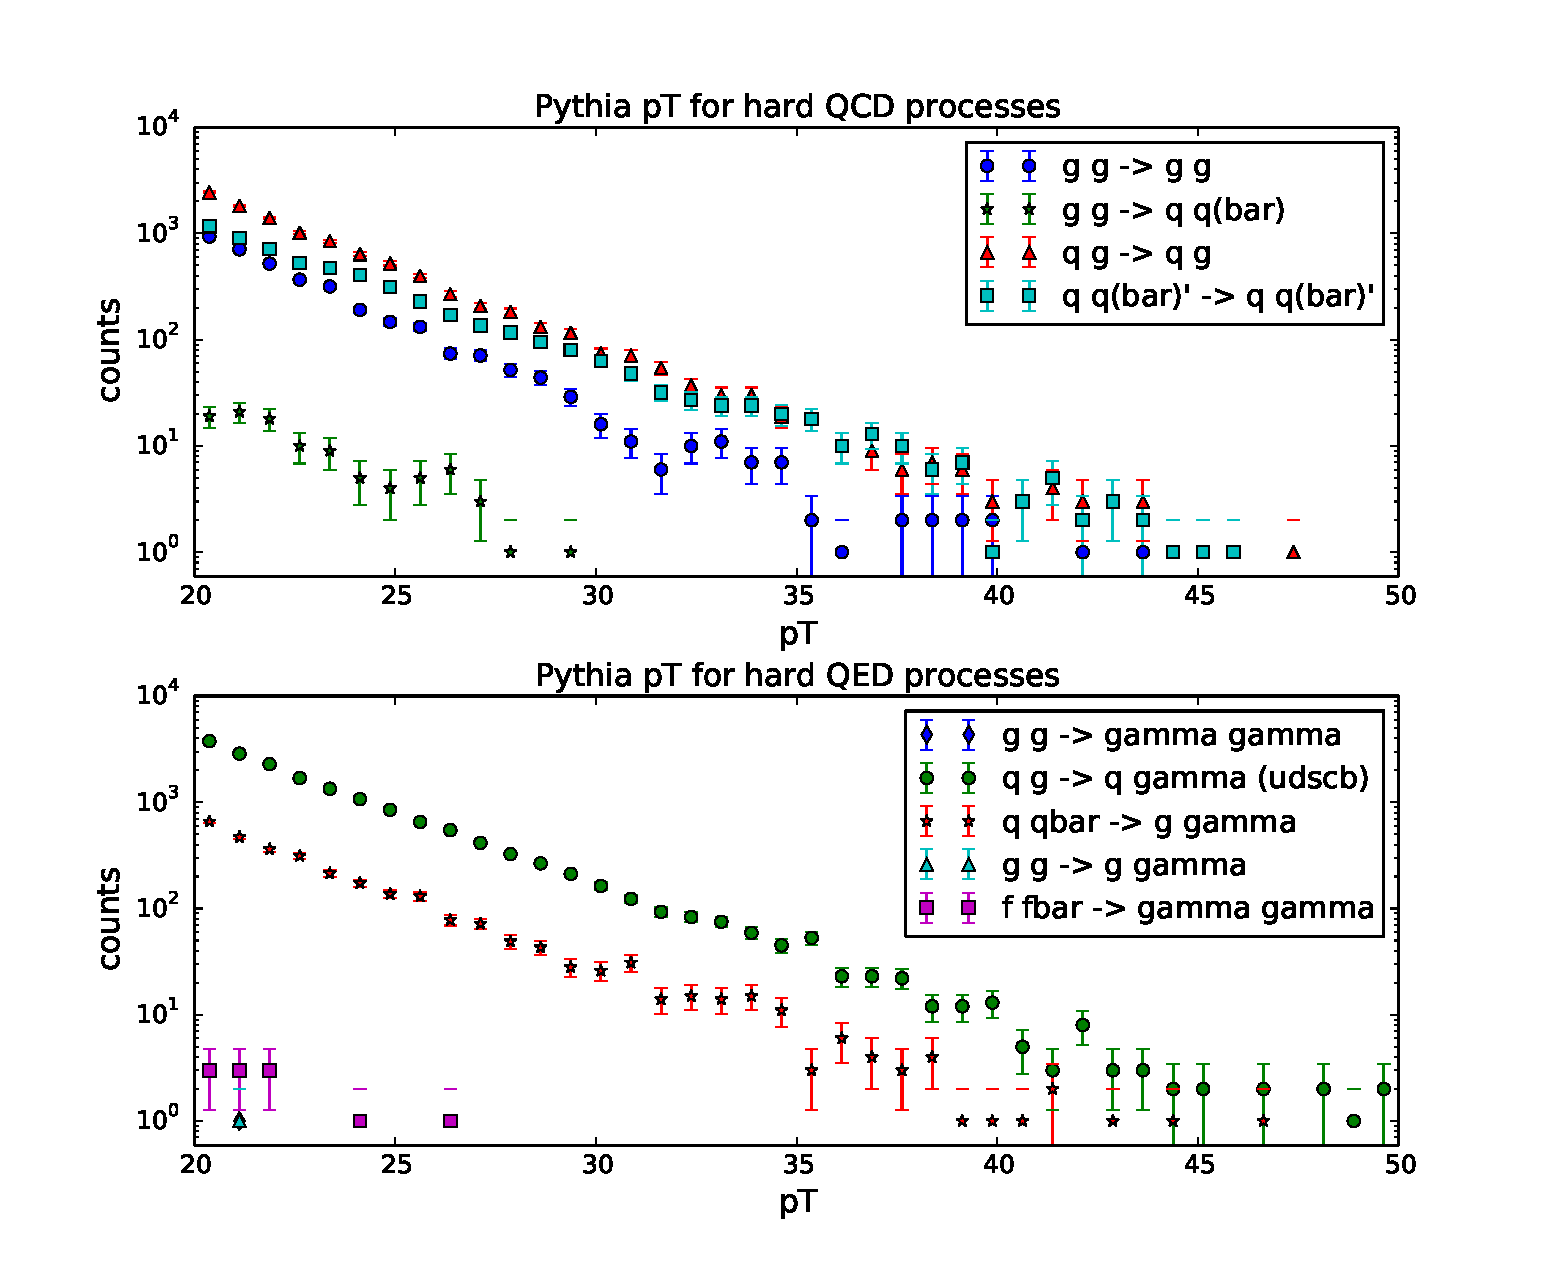
\includegraphics[width=0.9\textwidth]{pT_pythiaEvents.pdf}
\label{fig_label}
\caption{Distribution of jet pT for QCD and QED processes.  Figure created with [python pT_pythiaEvents.py -m 20000]}
\end{center}
\end{figure}

\begin{figure}[h]
\begin{center}
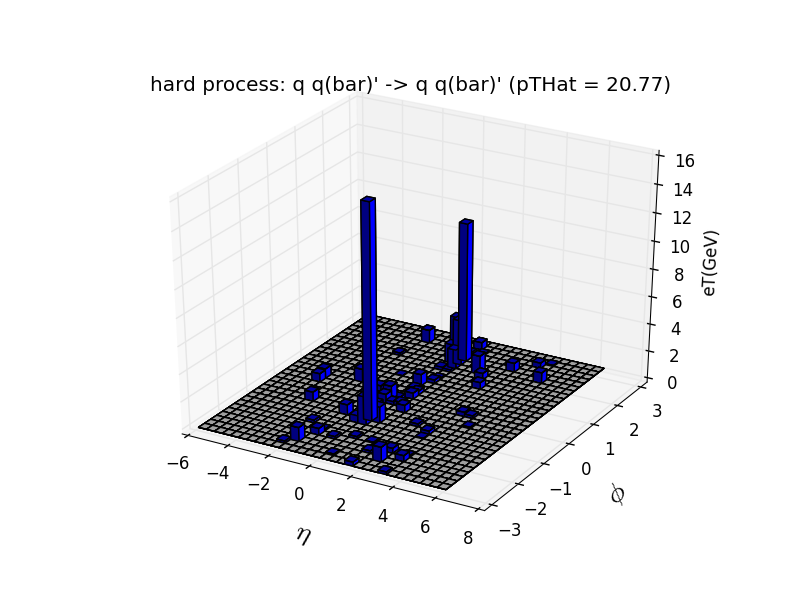
\includegraphics[width=0.9\textwidth]{2d_hist_jetplot.png}
\label{fig_label}
\caption{Pythia event display.  Figure created with [python 2d_hist_jetplot_wcol.py -o -b 30]}
\end{center}
\end{figure}

\section{Adding Trento Backgrounds}
%
% Describe how Trento is run, list parameters.
% Describe how we convert Trento output into particle number
% Explain how we generate pT, eta, and phi.
% Explain we add radial flow and elliptic flow from epsilon_2 variable.
%

\begin{figure}[h]
\begin{center}
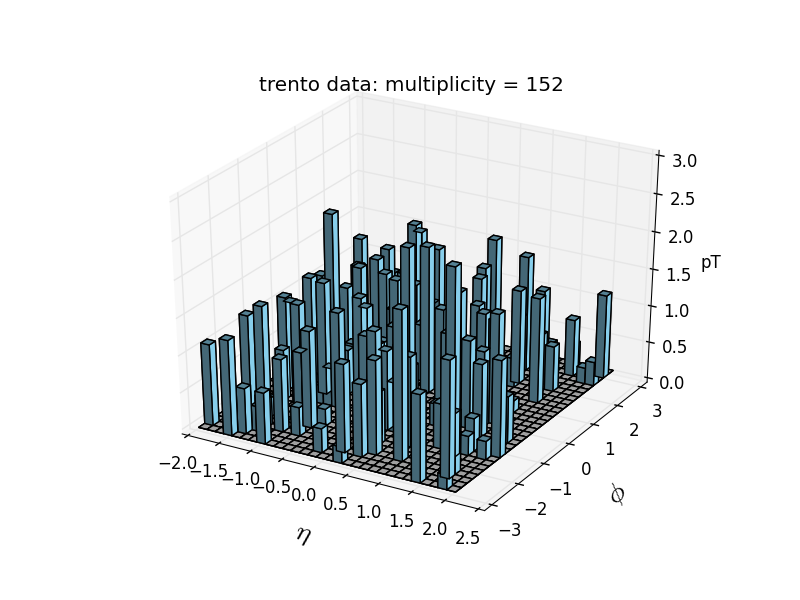
\includegraphics[width=0.9\textwidth]{2d_hist_trento.png}
\label{fig_label}
\caption{Trento event display (no jets).  Figure created with [python 2d_hist_trento.py -b 30]}
\end{center}
\end{figure}

\section{Working with SlowJet Finder}
%
% Describe SlowJet Finder algorithm and input parameters.
% Show examples of SlowJet Finder on Pythia only.
% Show example of SlowJet Finder on Pythia plus Trento.
%

\begin{figure}[h]
\begin{center}
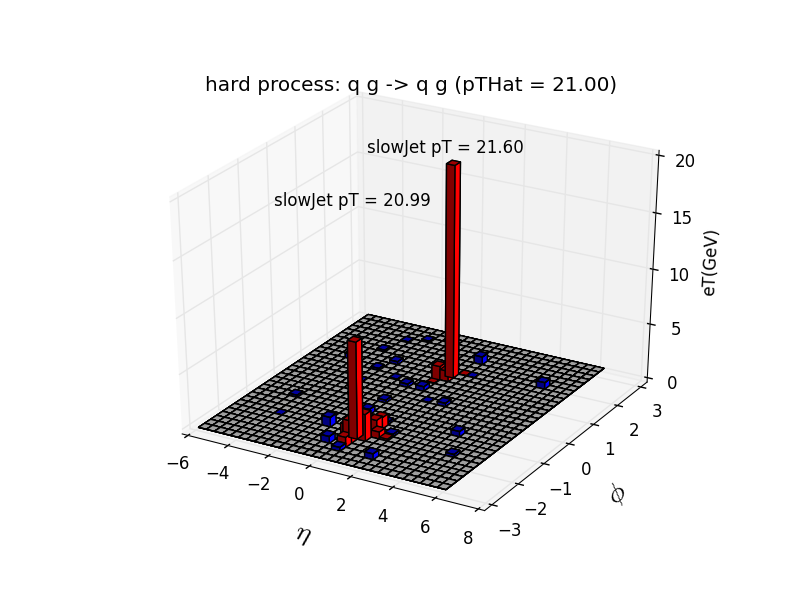
\includegraphics[width=0.9\textwidth]{2d_hist_jetplot_wcol.png}
\label{fig_label}
\caption{Event display for Pythia with SlowJet Finder.  Figure created with [python 2d_hist_jetplot_wcol.py -b 30]}
\end{center}
\end{figure}

\begin{figure}[h]
\begin{center}
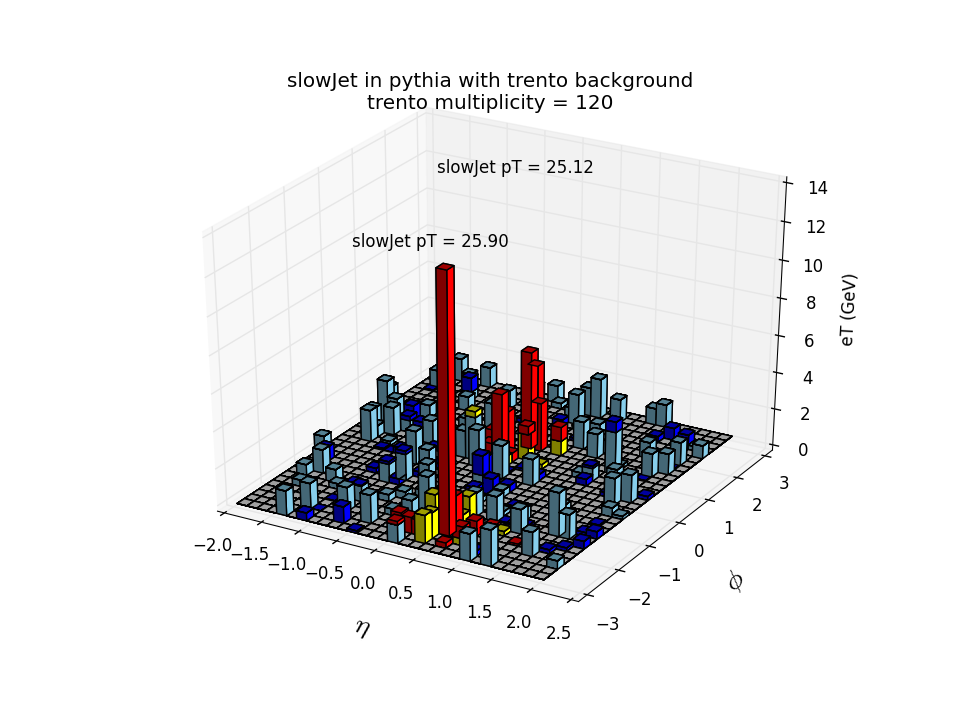
\includegraphics[width=0.9\textwidth]{pythia_slowjet_trento_hist1.png}
\label{fig_label}
\caption{Event display for Pythia+Trento with SlowJet Finder.  Figure created with [python pythia_slowjet_trento_hist.py -b 30 -s 1]}
\end{center}
\end{figure}

\begin{figure}[h]
\begin{center}
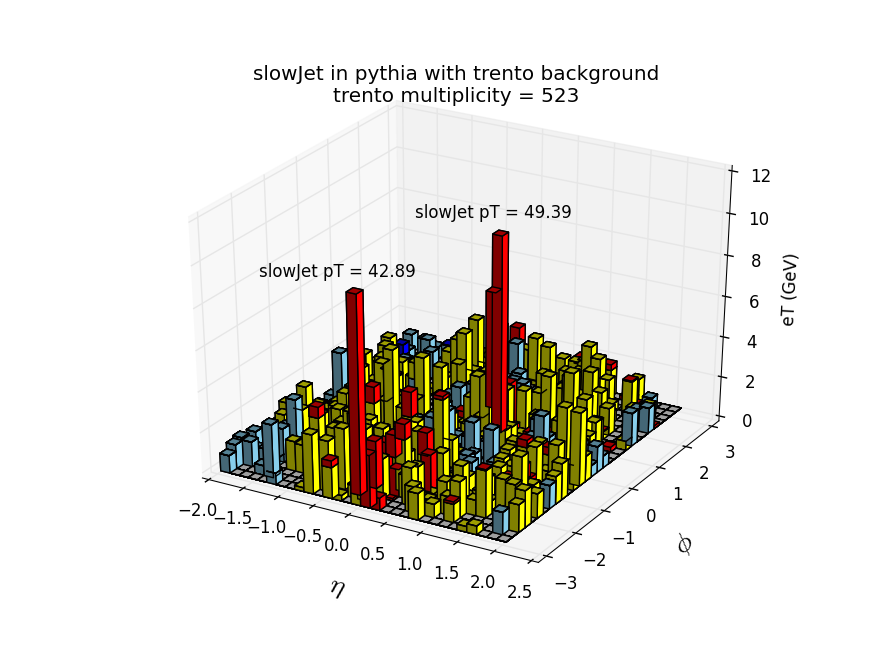
\includegraphics[width=0.9\textwidth]{pythia_slowjet_trento_hist2.png}
\label{fig_label}
\caption{Event display for Pythia+Trento with SlowJet Finder.  Figure created with [python pythia_slowjet_trento_hist.py -b 30 -s 1]}
\end{center}
\end{figure}

\section{Studying Jets}
%
% Define formula for fragmentation function.
% Explain methodology for tracing particles in 
%

\begin{figure}[h]
\begin{center}
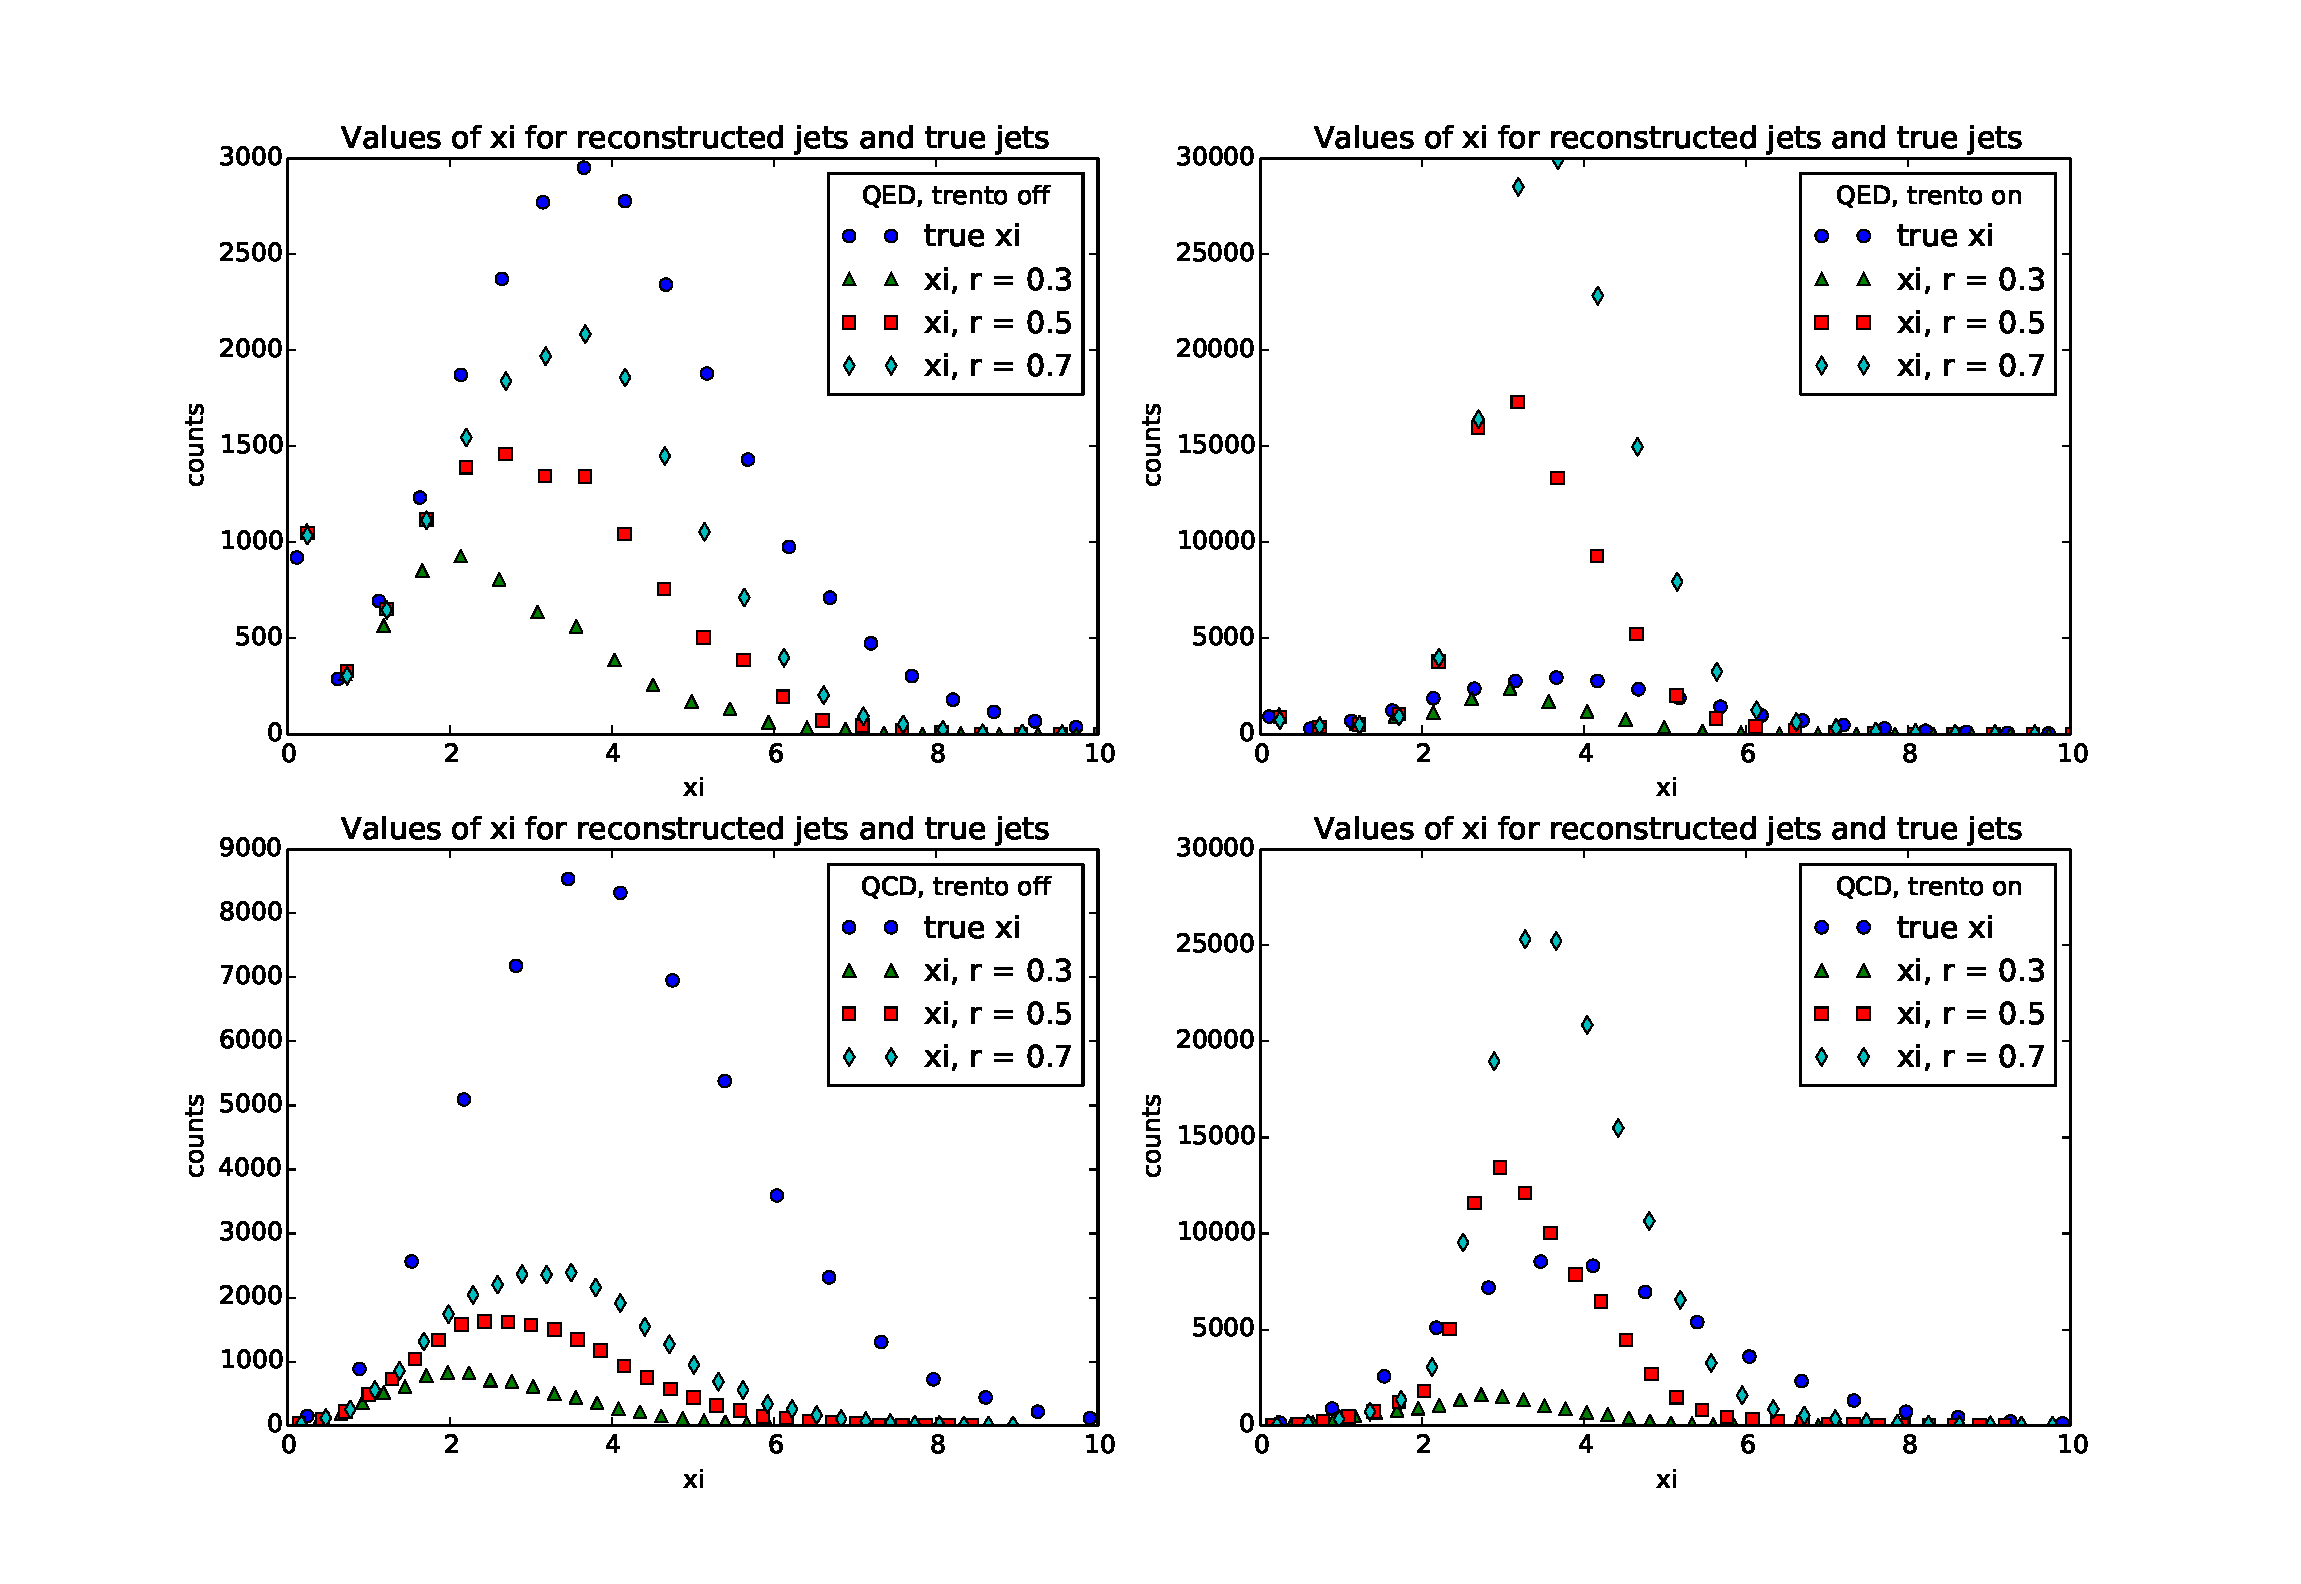
\includegraphics[width=0.9\textwidth]{compare_xi.pdf}
\label{fig_label}
\caption{Fragmentation Function (Xi) distributions for true and reconstructed QCD and QED jets, with and without trento backgrounds.  Figure created with [python compare_xi.py]}
\end{center}
\end{figure}

\appendix{Listing of Python Scripts}
%
% Provide descriptions for all python scripts, similar to README file.
%

\end{document}